\documentclass[times, utf8, zavrsni]{fer}
\setcounter{secnumdepth}{3}
\setcounter{tocdepth}{3}
\usepackage{booktabs}
\usepackage{algcompatible}
\usepackage{algorithm}
\begin{document}

% TODO: Navedite broj rada.
\thesisnumber{000}

\title{Izradra rasporeda laboratorijskih vježbi uporabom genetskog algoritma}

\author{Filip Pankretić}

\maketitle

% Ispis stranice s napomenom o umetanju izvornika rada. Uklonite naredbu \izvornik ako želite izbaciti tu stranicu.
\izvornik

% Dodavanje zahvale ili prazne stranice. Ako ne želite dodati zahvalu, naredbu ostavite radi prazne stranice.
\zahvala{Zahvaljujem se svojoj obitelji na svoj pružanoj podršci.}

\tableofcontents
\listoffigures

\chapter{Uvod}
Uvod rada. Nakon uvoda dolaze poglavlja u kojima se obrađuje tema.

\chapter{Problem raspoređivanja studenta u grupe}

U obrazovnim institucijama, dva najčešća problema slaganja rasporeda su dodjela grupa studentima te dodjela termina ispita. Raspored se smatra poželjnim ako profesor nema istovremeno dva predavanja, dva predmeta se istovremeno ne drže u istoj učionici, studenti nemaju više predavanja istovremeno te su zadovoljena sva stroga i što više blagih ograničenja. \citep{ganguli2017study}.

Za večinu problema raspoređivanja, pokazano je da su NP-teški\footnote{Ne postoji algoritam u polinomijalnom vremenu.} i da ne mogu biti rješeni u polinomnom vremenu koristeći detrministički algoritam. To vrijedi zbog kombinatorne eksplozije do koje dolazi zbog velikog broja, ograničenja, zahtjeva i velikog broja studenata, predemta, nastavnika i slično.

Prilikom izrade rasporeda potrebno je paziti na dvije vrste ograničenja: \emph{stroga ograničenja} \engl{hard constraints} i \emph{blaga ograničenja} \engl{soft contraints}.

\section{Stroga ograničenja}

Stroga ograničenja se odnose na probleme koji su fizički nemogući. Poput toga da je ili profesor ili student na dva ili više mjesta istovremeno. \citep{herath2017genetic}. Student mora imati dodjeljen samo jedan termin vježbi, taj termin se ne smije preklapati s drugim terminima. Profesori koji održavaju vježbe ne smiju istovremeno održavati dva ili više termina ali mogu imati dodjeljeno više termina u istom danu. U jednoj učionici se istovremeno može nalaziti samo jedna grupa studenata. Dodatne probleme mogu zadavati kapaciteti učionica, prilagođenost studentima s posebnim potrebama i slično.

\section{Blaga ograničenja}
Blaga ograničenja su ona koja se smatraju poželjnima, jutarnji termini, želje profesora za određenim predavaonama, termini predavanja slijedno bez višesatnih pauza između. Često se stroga ograničenja zbog specifičnih situacija mogu tretirati kao blaga. Na primjer kod predmeta s neobaveznom prisutnošću broj studenta se smanji nakon prvih nekoliko predavanja pa kršenjem maksimalnog kapaciteta ne nastaje veliki problem.

\chapter{Genetski algoritam}
\textbf{Evolucijsko računanje} je grana umjetne inteligencije koja se, najvećim dijelom, bavi rješavanjem optimizacijskih problema \citep{cupic-disertacija}. Evolucijsko računanje je familija metaheuristika\footnote{Skup algoritamskih koncepta primjenjivih na širok spektar problema} inspiriranih prirodnim procesima i biološkom evolucijom. Dijeli se na  3 grane: \emph{evolucijske algoritme}, \emph{algoritme rojeva} i \emph{ostalo}. 

\begin{figure}[htb]
\centering
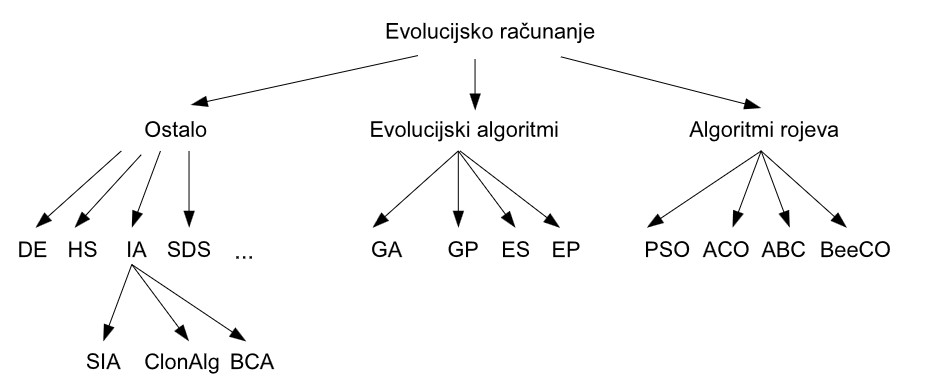
\includegraphics[width=15cm]{images/evolucijske_grane.png}
\caption{Podjela evolucijskog računanja na glavne grane uz odabrane algoritme. \citep{cupic-disertacija}}
\label{fig:evolucijske_grane}
\end{figure}

Evolucijski algoritmi su inspirirani Darwinovom teorijom o postanku vrsta koja se temelji na 5 pretpostavka:

\begin{enumerate}
	\item potomka uvijek ima više nego je potrebno,
	\item veličina populacije je prillbižno stalna,
	\item količina hrane je ograničena,
	\item kod vrsta koje se seksualno razmnožavaju, nema identičcnih jedinki već postoje varijacije te
	\item najveći dio varijacija prenos se nasljeđem.
\end{enumerate}

	\textbf{Genetski algoritam} jedan je od evolucijskih algoritama stvorenih za rješavanje optimizacijskih problema, a koji izravno utjelovljuje navedene postavke \citep{cupic-skripta}.  Klasični evolucijski algoritam sadrži sljedeće dijelove:
	
\begin{itemize}
	\item \textbf{Populacija} - podskup svih mogućih rješenja danog problema.
	\item \textbf{Jedinka} - jedno od rješenja u populaciji.
	\item \textbf{Funkcija dobrote} - numerička oznaka kvalitete neke jedinke.
	\item \textbf{Operator odabira roditelja} - operator odabira roditelja za daljnje križanje.
	\item \textbf{Operator križanja} - operator kombiniranja dviju jedinki kako bi se generirao jedan ili dva potomka.
	\item \textbf{Operator mutacija} - operator koji se koristi kako bi se održala raznolikost jedinki.
\end{itemize}

Sekvencijski\footnote{Rade u jednodretvenim sustavima} genetski algoritam može se podijeliti na dvije tipične izvedbe: \emph{eliminacijski genetski algoritam} \engl{steady-state genetic algorithm} te \emph{generacijski genetski algoritam} \engl{generational genetic algorithm} \citep{cupic-disertacija}. Kako se \emph{generacijski genetski algoritam} koristi za rješenje zadanog problema, njegov pseudokod je dan u nastavku:

\begin{algorithm}
\caption{Generacijski genetski algoritam}
\label{algo:generational-algo}
\begin{algorithmic}
\STATE{populacija := new jednika[N]}
\STATE{dobrota := new ocjena[N]}
\FOR{i := 0; i < N; i++}
\STATE{dobrota[i] := ocijeni(populacija[i])}
\ENDFOR
\WHILE{nije kraj}
\STATE{pom\_populacija := new jednika[N]}
\STATE{pom\_dobrota := new ocjena[N]}
\FOR{i := 0; i < N; i++}
\STATE{roditelj1 := odabirRoditelja(populacija)}
\STATE{roditelj2 := odabirRoditelja(populacija)}
\STATE{dijete := križaj(roditelj1, roditelj2)}
\ENDFOR
\algstore{generational-algo}
\end{algorithmic}
\end{algorithm}

\newpage

\begin{algorithm}
\begin{algorithmic}
\algrestore{generational-algo}
\STATE{populacija := pom\_populacija}
\STATE{dobrota := pom\_dobrota}
\ENDWHILE
\end{algorithmic}
\end{algorithm}

Kod generacijskog genetskog algoritma eventualno dobro dijete ne može se odmah iskoristiti; ono mora pričekati dok se ne završi čitava generacija.

Generacijski algoritam može taokđer biti elitistički\footnote{Svojstvo algoritma da sadrži najbolju jedinku}. Za razliku od ne elitističkih inačica, kroz evoluciju graf jedinki će biti nazubljen te najbolja jedinka nove generacije ne mora biti bolja od prethodne. \citep{cupic-skripta}

\chapter{Dodjela termina laboratorijskih vježbi}
\label{ch:glavni}

Problem dodjele termina laboratorijskih vježbi znatno je lakši od izrade cjelovitog rasporeda. Nasuprot originalnog problema izrade cjelovitog rasporeda, sad postoji već prethodno izrađen raspored te je isti potrebno popuniti dodatnim terminima laboratorijskih vježbi. Također, nije potrebno uzeti u obzir cijeli raspored već samo jedan tjedan u semestru, što znatno olakšava problem i sami pristup problemu. Nadalje, nije potrebno pratiti niti sljedeće stavke: željeni termini profesora ili asistenata, profesori ili asistenti dodijeljeni terminu, održavaju li se dva ili više termina istovremeno itd. Općenito je potrebno paziti na navedena ograničenja, ali sada ne spadaju u opseg ovog rada.

\section{Reprezentacija rasporeda u obliku jedinke}

Svaki generirani raspored (također istoznačno: jedinka) potrebno je ispravno prikazati u memoriji. Ovisno o zapisu koji se koristi problem može znatno olakšati ili otežati. Osim zapisa same jedinke program prima niz datoteka potrebnih za rad algoritma: popis studenata, popis dostupnih termina laboratorijskih vježbi, maksimalan i minimalan broj studenata po terminu te prethodna zauzetost studenata.

Prvo je potrebno definirati univerzalne podatke koji se koriste neovisno o zapisu samog rasporeda. Zapis termina laboratorijskih vježbi dan je formatu:

\emph{šifra\_termina;kapacitet;datum;vrijeme\_početaka;vrijeme\_kraja;učiona}, gdje je dodatno \emph{kapacitet} u formatu: \emph{makimalan\_kapacitet/minimalan\_kapacitet}. Svaki zapis spremamo u četiri odvojena niza: niz s cijelovitim zapiso, niz s početkom termina, niz s krajem termina i niz s datumom termina. Nadalje se termini referenciraju indeksom na kojem su raspoređeni.

Slijedi prikaz termina studenata. Moguće je da u tablici zauzetosti studenata se nalaze studenti kojima nije potrebno dodijeliti termin. Stoga se za prikaz rasporeda koristi tablica raspršenog adresiranja\footnote{Struktura podataka koja u pretincima adresiranim nekim ključem sadrži određeni tip podatka.} koja kao ključ prima JMBAG\footnote{Jedinstveni matični broj akademskog građanina} studenta, a kao vrijednost sadrži istu prima koja sada kao ključ prima datum termina a kao vrijednost ima strukturu podataka vektor\footnote{Struktura podataka koji automatski alocira i dealocira memoriju, a ponaša se kao niz} s popisom prethodnih termina. Slijedni termini se spajaju u jedan zajednički termin kako bi se kasnije ubrzala provjera kolizija. Kolizije već prethodno dodijeljenih termina prilikom učitavanja podataka se ne provjeravaju.

\begin{figure}[htb]
\centering
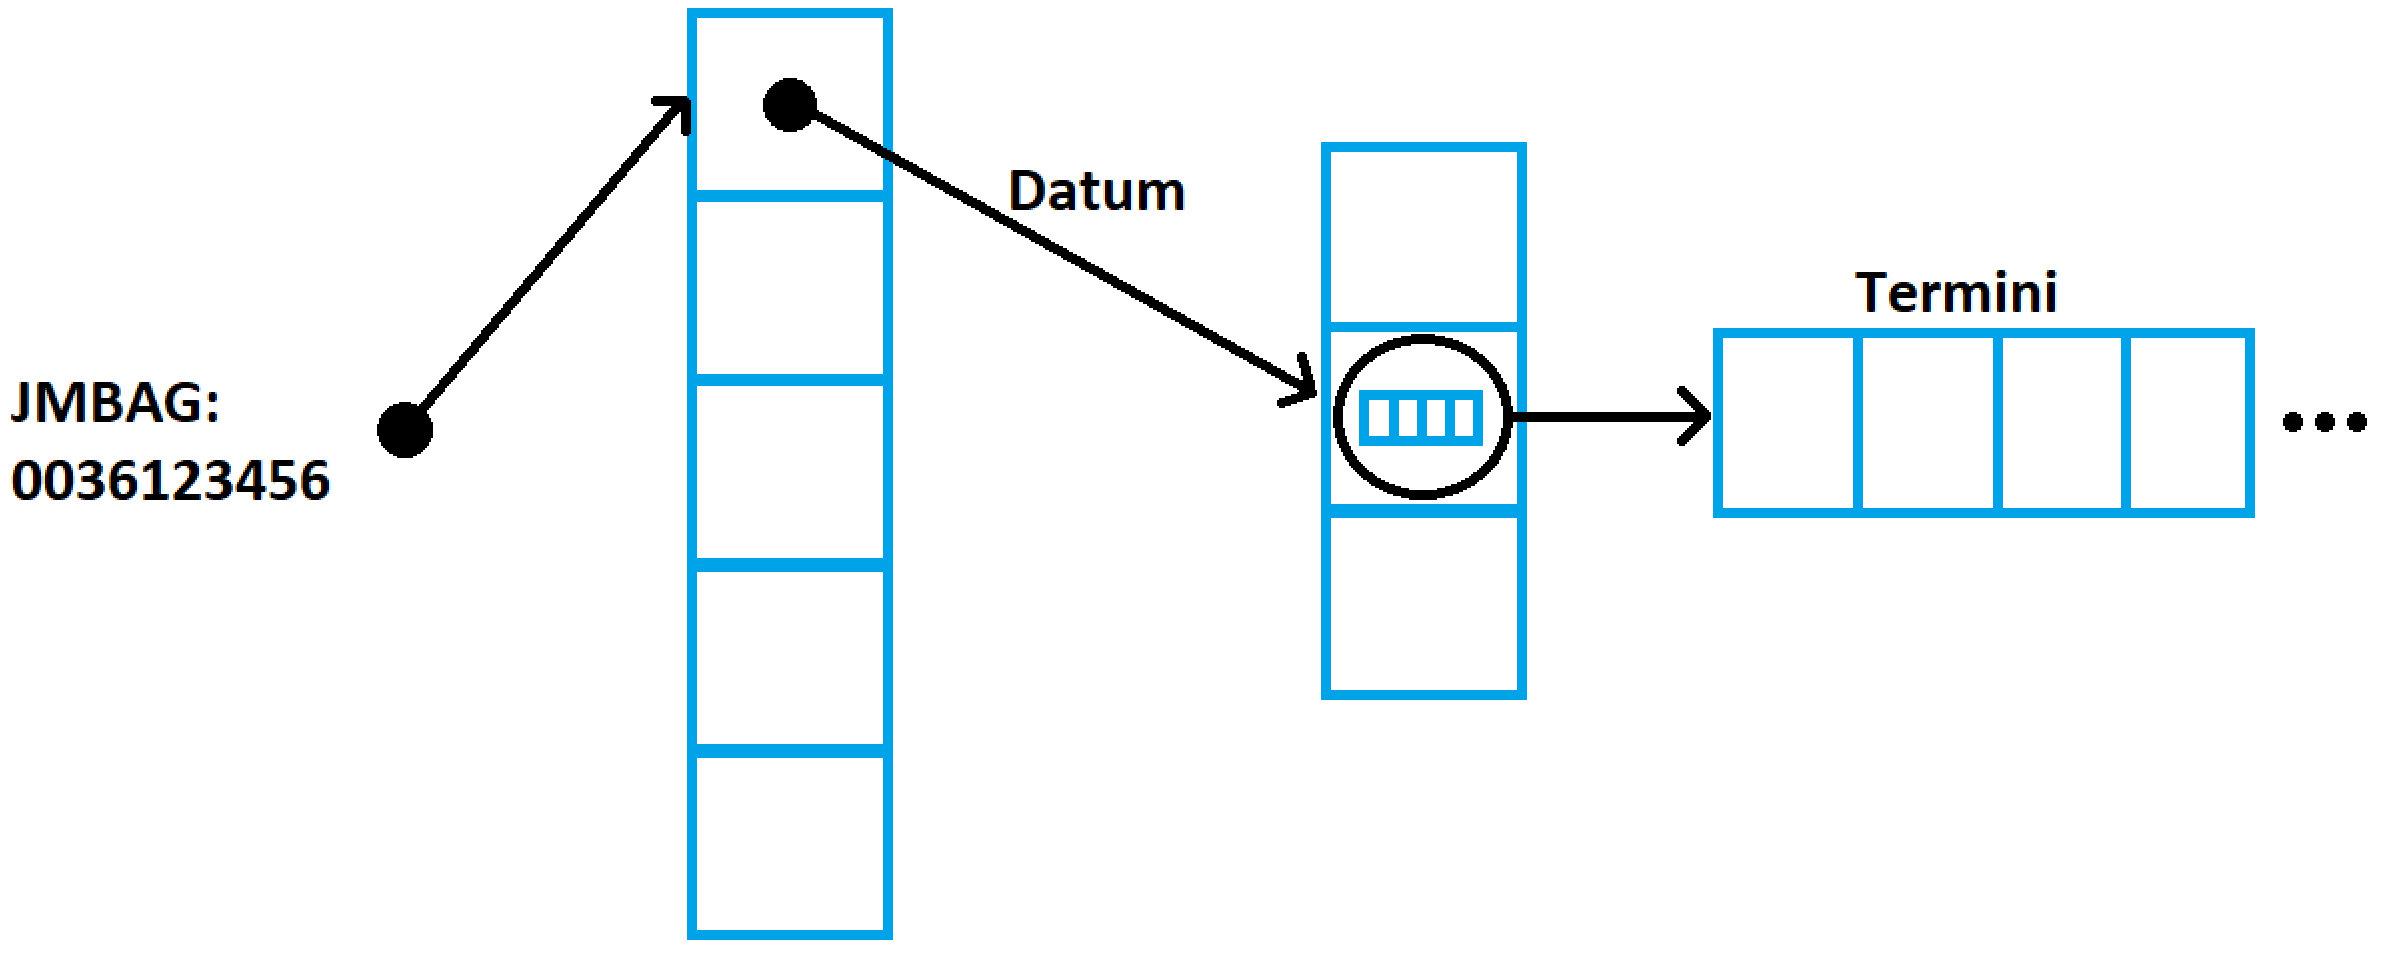
\includegraphics[width=15cm]{images/prikaz_termina.png}
\caption{Prikaz zapisa nastavnih obveza studenta u memoriji.}
\label{fig:prikaz_termina}
\end{figure}

Popis studenata kojima je potrebno dodijeliti termin mogu sadržavati termin koji ne postoji u tablici prethodno dodijeljenih termina, u tom slučaju se pretpostavlja da student u tom tjednu nema ostalih nastavnih obveza. Studenti se prikazuju kao niz JMBAG-a kojemu se kasnije pristupa preko indeksa pojedinog elemenata.

Dva načina zapisa rasporeda koja će biti obrađena su \emph{niz termina s listom studenta} i \emph{niz studenta s dodijeljenim terminom}.

\subsection{Niz termina s listom studenata}

Prvi način zapisa je niza termina gdje svaki element tog niza sadrži vektor sa studentima kojima je dodijeljen taj termin.

\begin{figure}[htb]
\centering
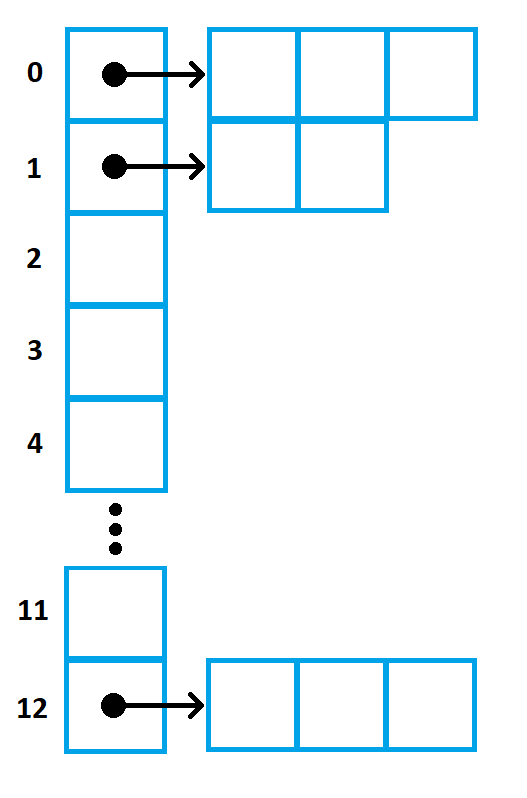
\includegraphics[width=7cm]{images/prikaz_jednike_1.png}
\caption{Prikaz niza termina s listom studenata u memoriji.}
\label{fig:prikaz_jednike_1}
\end{figure}

Prednosti ovog zapisa su lakši ispis podataka jer svaki termin odmah sadrži popis studenata i jednostavnija provjera zauzetog kapaciteta nekog termina. Prednosti je vrlo malo, dok mana ima puno više.

Neki od nedostataka su da je potrebno je paziti da je svaki student dodijeljen samo jednom terminu, teže je implementirati operatore mutacije i operator križanja jer jedinka ima dvije osi od kojih je jedna varijabila, također je zbog toga otežan izračun preklapanja. Dodatno, ovaj prikaz je i memorijski i vremenski zahtjevan zbog dodatnog korištenja struktura podataka.

\subsection{Niz studenta s dodijeljenim terminom}

Druga način prikaza je niz gdje indeks svakog elementa predstavlja jednog studenta, a element je indeks dodijeljenog termina.

Ovaj način pruža jednodimenzionalni niz što znatno olakšava definiranje operatora križanja i mutacije. Kako svaki student predstavlja jedan element niza, odmah je riješeno tvrdo ograničenje da student može pristupiti samo jednom terminu laboratorijskih vježbi. Lakše je izračunati pojedina preklapanja jer jednostavno pronaći za svakog studenta pronaći dodijeljeni termin. Memorijski i vremenski je efikasniji od prvog načina zbog jednostavnije strukture.

Otežan je izračun zauzetog broja mjesta po terminu i ispis podataka. Za provjeru zauzeća potrebno je jednom proći  kroz cijeli niz kako bi se za svaki termin prebrojala zauzeta mjesta, a za ispis rasporeda je potrebno za svaki termin proći kroz cijeli niz te ispisati studenta kako se naiđe na njega ili je potrebno u zasebnoj strukturu držati popis studenata slično kao prvi zapis. Kako se raspored ispisuje samo povremeno, to onda više nije problem.

\begin{figure}[htb]
\centering
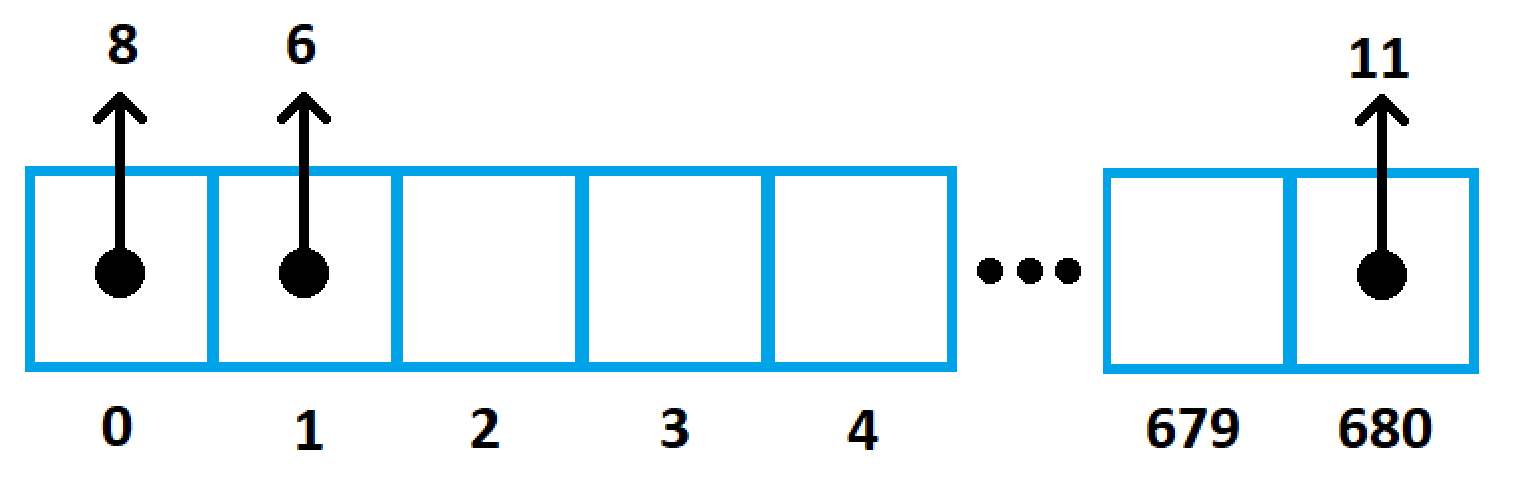
\includegraphics[width=13cm]{images/prikaz_jednike_2.png}
\caption{Prikaz niza termina s listom studenata u memoriji.}
\label{fig:prikaz_jednike_2}
\end{figure}

Zbog velikog broja prednosti druge strukture naspram prve, ta struktura je odabrana za prikaz rasporeda.

\section{Ocijena rasporeda}

Ocjena rasporeda je rezultat funkcije dobrote \engl{fitness}. Točnije to je numerička oznaka koja se koristi za ocjenu kvaliteta rasporeda. Ukupna ocjena nekog rasporeda jednaka je sumi funkcija dobrote za svakog studenata iz nekog rasporeda.

\begin{equation}
\sum_{i=0}^{n} dobrota(student[i])
\label{eq:dobrota}
\end{equation}

\subsection{Dobrota i kazna}

Osim dobrote, raspored može koristiti i kaznu \engl{punishment}. Kazna je mjera koliko je koliko je neki raspored loš. Ponekad je za neki problem lakše definirati ukupnu kaznu, nego ukupnu dobrotu. U praksi se pokušava ili minimizirati kazna ili maksimizirati dobrota. Kazna isto kao i dobrota je zapravo heuristika koja aproksimira koliko je daleko odnosno blizu dobiveno rješenje od cilja tj.\ najboljeg rješenja.

U sklopu ovo rada, najbitnije svojstvo rasporeda je da nema preklapanja, stoga će bolji raspored biti onaj koji ima manje preklapanja, a nadalje onaj koja ima bolju ocjenu.

Prilikom izračuna ocijene rasporeda, sljedeća svojstva su uzeta kao pretpostavke:

\begin{itemize}
	\item studenti preferiraju imati vježbe u istom danu kad već imaju nastavne aktivnosti,
	\item bolji je termin koji stvara manju rupu do najbliže nastave aktivnosti nego onaj koji stvara veću,
	\item broj nastalih pauza u rasporedu nije bitan i 
	\item bolji je termin koji je slijedno s nastavnim aktivnostima bez pauze neovisno o opterećenju taj dan
\end{itemize}

\subsubsection{Dobrota}

Ako bi raspored koristio dobrotu za svoju ocjenu, neke od heuristike koje bi mogli koristiti su broj studenata koji nemaju preklapanje i broj studenata kojima je dodijeljen termin slijedno s ostalim nastavnim aktivnostima.

Teško je definirati kvalitetnu funkciju dobrote, jer je vrlo malo svojstva kojima se može dodijeliti smislena numerička vrijednost. Čak i ako se uspiju pronaći smislene karakteristike za funkciju dobrote, teško je namjestiti vrijednosti tako da algoritam preferira sva svojstva istovremeno.

Na primjer ako se za svakog studenta bez preklapanja funkcija dobrote poveća za 10, a za svaki slijedni raspored se poveća za 5. Algoritam će vrlo vjerojatno preferirati studente koji nemaju preklapanja te neće preferirati da studenti imaju slijedna predavanja. Opet može se dogoditi da algoritam sve studente stavi u par termina gdje svi studenti imaju slijedna predavanja ali s puno preklapanja i puno prekršenih ograničenja.

\subsubsection{Kazna}

Rasporedi sati esencijalno imaju jako puno ograničenja koja ne smiju biti prekršena ili smiju ali do neke granice. Stoga je lakše implementirati funkciju kazne rasporeda. Za kaznu isto kao i za dobrotu vrijedi da ako se psotavi prevelika kazna za bilo koje svojstvno, vjerojatno je da će dominirati rasporedi koji imaju minimiziranu kaznu s tim svojstvom.

Naime, kako je cilj pronaći raspored koji nema preklapanja to ne predstavalja preveliki problem, ali ako se koristi kazna umjesto dobrote za ocjenu algoritma, dostupan je puno veći broj heuristika koje mogu potencijalno pronaći kvalitetniji raspored.

Neke od heuristika koje su dostupne su: broj preklapanja, broj rupa, vrijeme preklapanja, koliko je studenata premalo ili previše u nekom terminu i vremenski period najmanje rupe nastale nakon dodavanja termina.

\subsubsection{Kazna s kombinacijom dobrote}
\label{sec:kombinacija}

Kao najbolja opcija se ipak pokazala kazna s kombinacijom dobrote. Osim heuristika kazne uvodi se mali broj heuristika koje rasporedu daju nagradu, to jest smanjuju kaznu za iznos pomnožen malim koeficijentom ako su zadovoljena neka dobra svojstva. Kada bi nagrada bila velika, onda bi efektivno algoritam pokušavao maksimizirati nagradu umjesto da minimizira kaznu.

\subsection{Ograničenje broja studenata}

Kod izračuna cijene prilikom kršenja maksimalnog ili minimalnog kapaciteta koriste se sljedeće pretpostavke:

\begin{itemize}
	\item minimalni broj studenata u terminu je uvijek 15,
	\item maksimalan broj studenata u terminu je uvijek 16,
	\item lošije je kada broj studenata premaši maksimalan kapacitet, nego kad je broj studenta manji od minimuma.
\end{itemize}

Nakon što je dostupna informacija o broju studenata za svaki termin, dodjeljuje se kazna ovisno o prekršenim ograničenjima. Kazna za termine kojima je dodijeljen veći broj studenata od maksimalnog jednaka je razlici broja dodijeljenih studenata i maksimalnog broja studenata za taj termin pomnožena s nekim koeficijentom.

Nakon što je dostupna informacija o broju studenata za svaki termin, dodijeljuje se kazna ovisno o prekršenim ograničenjima. Kazna za termine kojima je dodijeljen veći broj studenata od maksimalnog jednaka je razlici broja dodijeljenih studenata i maksimalnog broja studenata za taj termin pomožena s nekim koeficijentom.

\begin{equation}
(brojStudenata - 16) \cdot koeficijentZaViseStudenata
\label{eq:max-studenta}
\end{equation}

Istovjetno, termini kojima je dodijeljen manji broj studenata od minimalnog doprinose kaznom jednakom razlici minimalnog broja studenata i dodijeljenog broja studenata pomnoženom s nekim koeficijentom.

\begin{equation}
(15 - brojStudenata) \cdot koeficijentZaManjeStudenata
\label{eq:min-studenta}
\end{equation}

Koeficijent za manji i veći broj studenata nisu jednaki, što se temelji na trećoj zadanoj pretpostavci. Nastavniku je očigledno jednostavnije ispitati manji broj studenata od minimuma, nego veći od maksimuma, zato je koeficijent za manje studenata manji od onog za više. Dobro svojstvo za ta dva koeficijenta je da njihova razlika ne bude prevelika. Jer ako bi koeficijent za manji broj studenata bio premali onda bi algoritam mogao dominirati rasporedima koji nemaju popunjena sva mjesta u učionicama, a isto vrijedi i za obrat.

\subsection{Izračun preklapanja}

Student može imati preklapanja u rasporedu prije nego li mu je dodijeljen termin laboratorijskih vježbi. Kod takvih situacija se računaju zasebno kolizije dodijeljenog termina sa svakim prethodnim terminom zasebno, tako da teoretski jedan student može proizvesti više od jedne kolizije. Kazna se dodjeljuje svakoj od tih kolizija kako bi se čak i u slučaju kolizija što prije odbacio raspored gdje pojedinim studentima gotovo pa nije moguće pristupiti terminu laboratorijskih vježbi.

Preklapanje dvaju termina lako se može provjeriti formulom:

\begin{equation}
max(t1, T1) - min(t0, T0) < (t1 - t0) + (T1  - T0)
\label{eq:preklapanje}
\end{equation}

\emph{T0} i \emph{T1} predstavljaju redom početak i kraj dodijeljenog termina, a \emph{t0} i \emph{t1} redom početak i kraj nekog od termina ostalih nastavnih obveza. \emph{max(t1, T1) - min(t0, T0)} predstavlja interval na kojem se nalaze na kojem se nalaze termini koji se trenutno uspoređuju te ako je taj interval manji od zbroja duljina zasebnih intervala, onda postoji preklapanje.

\begin{figure}[htb]
\centering
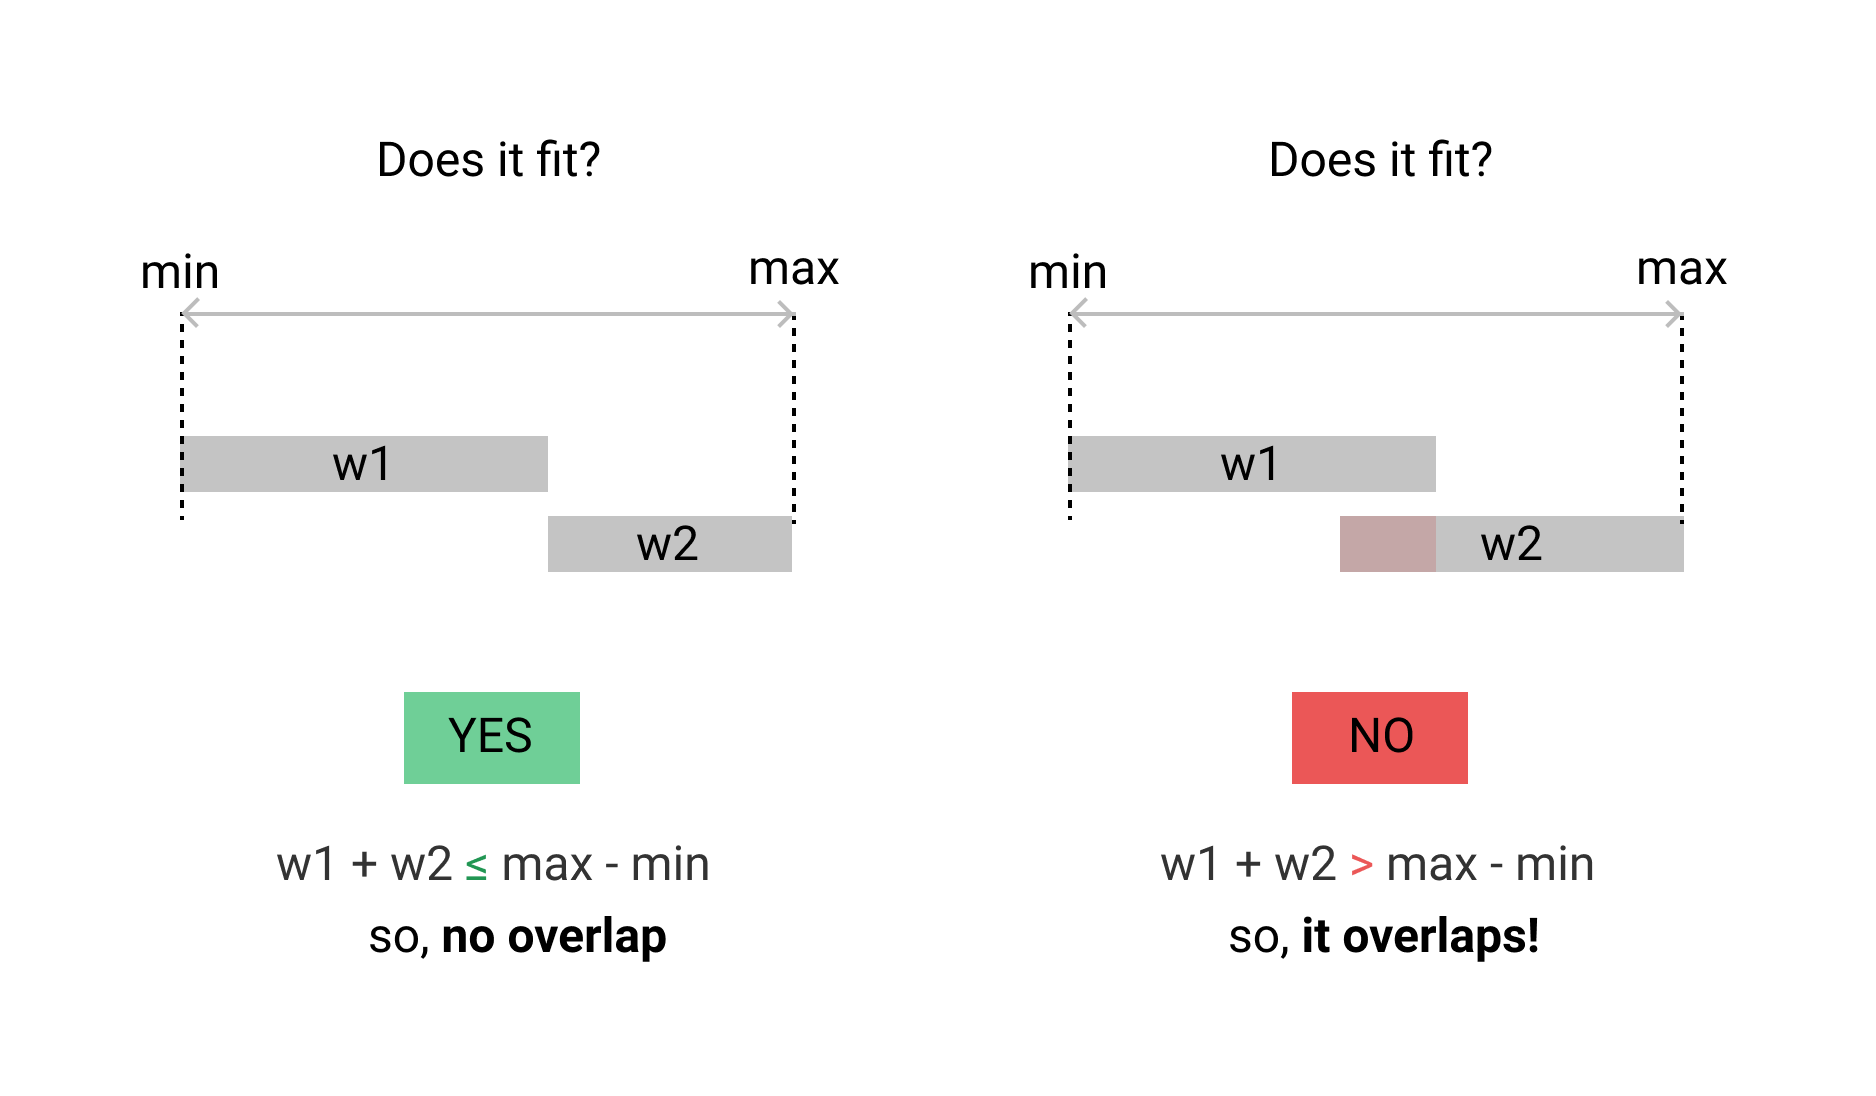
\includegraphics[width=15cm]{images/preklapanja.png}
\caption{Provjera preklapanja dva termina.}
\label{fig:preklapanja}
\end{figure}

Najvažnije svojstveno rasporeda je da ima minimalni broj preklapanja zato se umnožak preklapanja množi s koeficijentom koji je veći od ostalih. Razlog tome je kako bi se što prije pronašao raspored koji ima minimalan broj preklapanja te onda krenulo u dodatno poboljšanje ostalih svojstva rasporeda.

\subsection{Slijedni termini}

Kao što je spomenuto u odjeljku \ref{sec:kombinacija}, zbog nekih poželjnih svojstva rasporedu se može dodijeliti nagrada. Nagrada je implementirano tako da ukupnu kaznu rasporeda smanji za neku brojčanu konstantu. Manje konstante osiguravaju, pogotovo ako je implementirano više nagrada, da se ne preferiraju rasporedi s više nagrada i manje prekršenih ograničenja. 

Jedno od tih svojstva je slijedno održavanje termina. Sljednost se provjerava samo ako se navedeni termin ne preklapa s niti jednim ostalim terminom. Za provjeru sljednosti može se koristiti formula \ref{eq:preklapanje} ali tako da se znak nejednakosti promjeni u znak jednakosti.

\begin{equation}
max(t1, T1) - min(t0, T0) = (t1 - t0) + (T1  - T0)
\label{eq:slijednost-long}
\end{equation}

Ali, zbog toga što provjera sljednosti ponovo uspoređuje dobiveni termin sa svim ostalim terminima, poželjno je ako je moguće ubrzati provjeru. Pa se zato za provjeru preklapanje dva termina koristi sljedeća formula:

\begin{equation}
t0 = T1 \lor T0 = t1
\label{eq:slijednost-short}
\end{equation}

gdje \emph{T0, T1, t0} i \emph{t1} imaju isto značenje kao i formula \ref{eq:preklapanje}. Dovoljno je samo provjeriti počinje li ili završava li dodijeljeni termin onda kada bilo koji drugi redom završava ili počinje.

\subsection{Pauza nastala nakon dodijeljenog termina}

Broj pauza u rasporedu nije bitan, već se za izračun kazne koristi samo minimalna udaljenost dodijeljenog termina do svih ostalih termina. Provjera pauza se ne vrši u slučaju da su već pronađena dva slijedna termina ili ako postoji kolizija. Za pronalazak najmanjeg perioda pauze u rasporedu koristi se sljedeća formula:

\begin{equation}
min(|T0 - t1|, |T1 - t0|)
\label{eq:min-rupa}
\end{equation}

gdje \emph{T0, T1, t0} i \emph{t1} imaju isto značenje kao i formula \ref{eq:preklapanje}. Potom se kazna povećava za iznos izračunat formulom:

\begin{equation}
koeficijent \cdot najmanjiRazmak^2
\label{eq:min-rupa-kazna}
\end{equation}

Koeficijent služi za podešavanje doprinosa kazne. Prema pretpostavci bolji je raspored onaj koji nema pauze znači da će rasporedi s većom pauzom biti gori, tj. imat će veću kaznu. Kako bi se ta pauza što više minimizirala, najmanji razmak se kvadrira kako bi se studentima dodijelili termini sa što manjim vremenskim razmakom.

\subsection{Termin dodjeljen u danu bez nastavnih obveza}

Temeljeno na prvoj pretpostavci izračuna ocjene rasporeda, studenti preferiraju termine laboratorijskih vježbi u istom dana kada imaju neku drug nastavnu aktivnost, stoga ako student nema drugih nastavnih aktivnosti u danu održavanja laboratorijskih vježbi, dodjeljuje se kazna relativno velikog iznosa.

Provjera ima li student neke druge nastavne aktivnosti taj da ili ne održava se na samom početku prije provjera preklapanja, sljednosti termina i pauze s najmanjim vremenskim razmakom. Ako je ta provjera istina onda se ostala svojstva ne provjeravaju.

\section{Elitizam}

\textbf{Elitizam} \engl{elitism} je svojstvno algoritma da uvijek sadržava najbolju jedinku.

Odabir elitnog rasporeda vrši se tako da se prolazi kroz kazne svih jedinki i gleda se ima li raspored manji broj preklapanja od prethodnoga potom. U slučaju da ima, raspored na kojeg se naišlo se bira kao elitni, a u slučaju da je broj preklapanja jedinak onda se odabire onaj s manjom kaznom.

Kod elitističkih algoritama graf koji prikazuje kretanje funkcije kazne kroz evoluciju je monoton. Zbog načina odabira elitinog rasporeda, ovdje će to svojstvo monotonosti biti vidljivo oko 1000-te iteracije kada broj preklapanja postane 0.

\begin{figure}[htb]
\centering
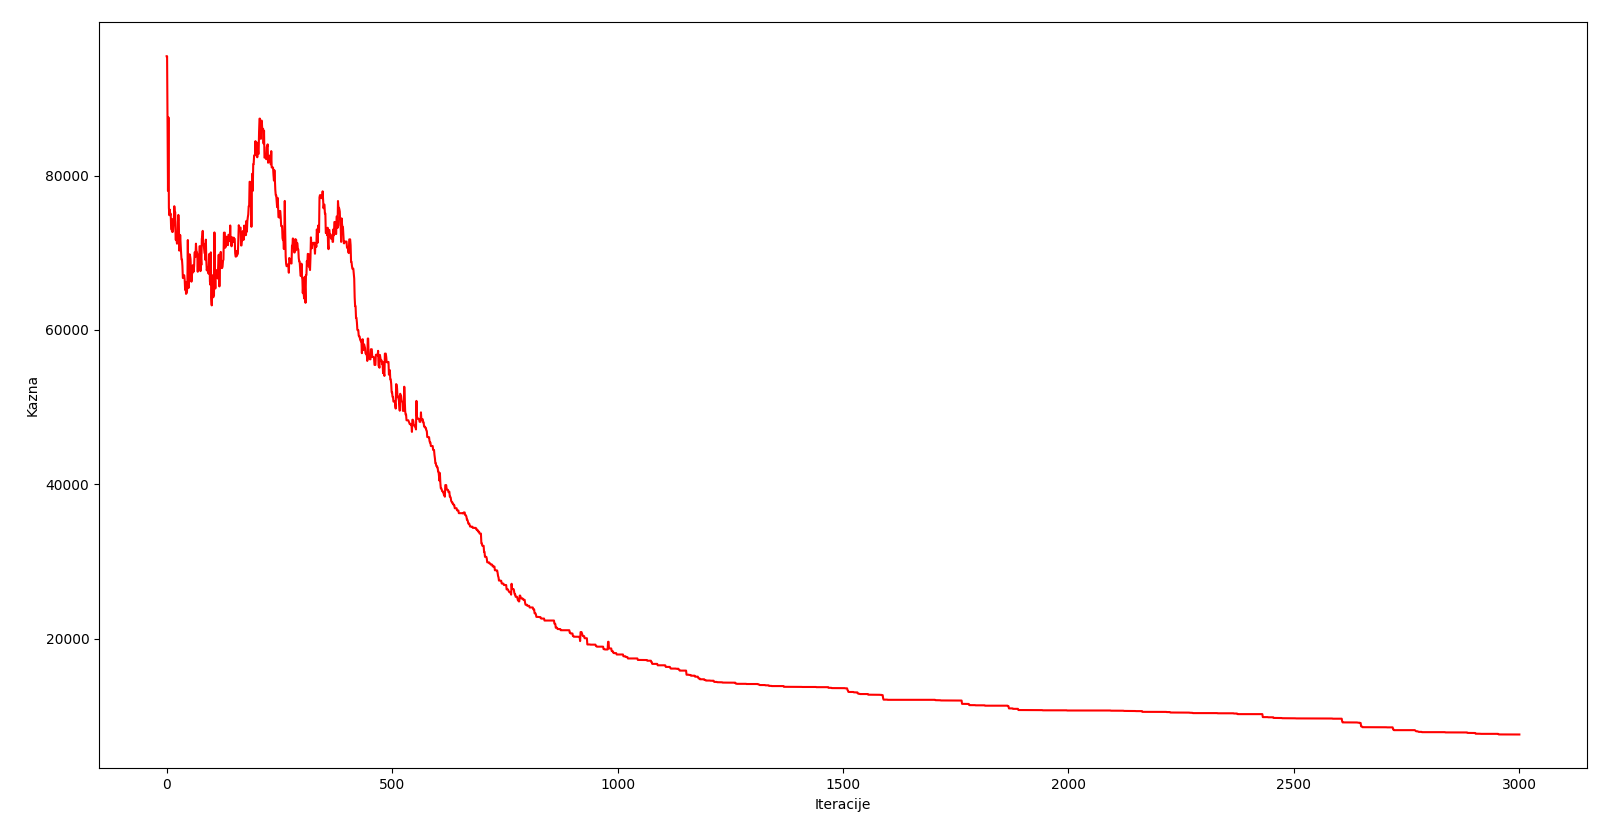
\includegraphics[width=14cm]{images/elitizam_da.png}
\caption{Generirani raspored s uključenim elitizmom.}
\label{fig:elitiziam_da}
\end{figure}

Kod algoritama koji nisu elitistički taj će graf biti nazubljen: prosječne vrijednosti funkcije kazne asimptotski će padati ali je sasvim moguće da u nekon koraku algoritma kazna najbolje jedinke bude veća kazne najbolje jedinke koju je algoritam imao u nekom prethodnom koraku \citep{cupic-skripta}.

\begin{figure}[htb]
\centering
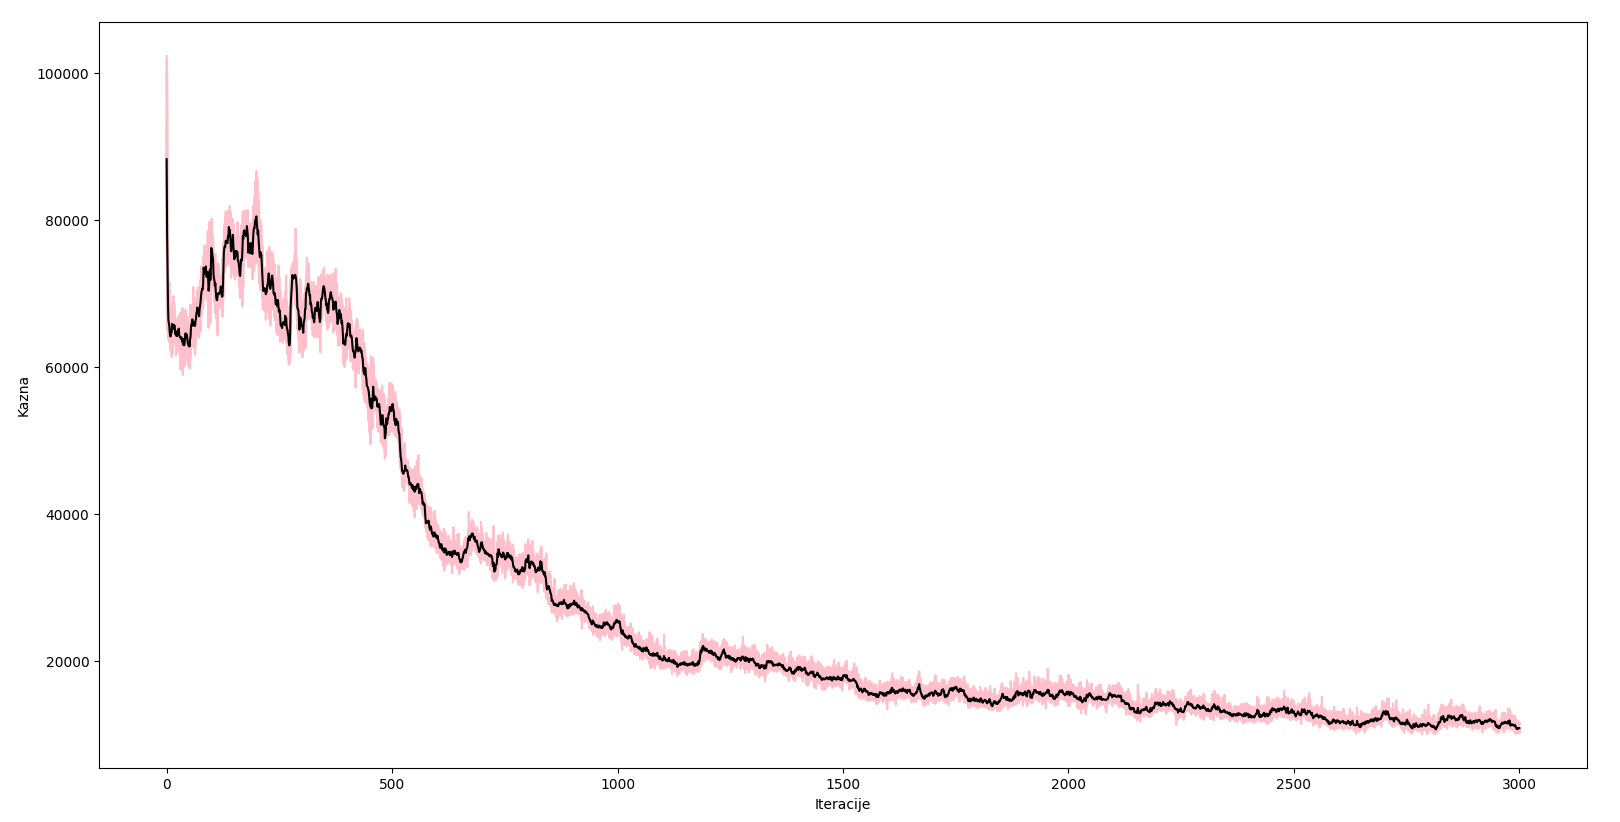
\includegraphics[width=14cm]{images/elitizam_ne.png}
\caption{Generirani rasporedi s isključenim elitizmom.}
\label{fig:elitiziam_da}
\end{figure}

Prilikom izrade rasporeda očuvanje elitnog rasporeda je pokazalo dobra svojstva poput brže konvergencije i manjeg raspršenja. A kod nekih postavka algoritma, jedino su s uključenim elitizmom rasporedi počeli konvergirati. To je zato što elitni raspored pruža algoritmu točku za koju se može držati kako bi se odupro divergenciji zbog raznih loših utjecaja na algoritam. Time algoritam postaje striktno konvergentan.

\section{Odabir roditelja}

Kod odabira roditelja važno je da oba roditelja budu različita kako bi se održala raznolikost rasporeda. Kada bi oba odabrana roditelja bila jednaka, raspored nastao operatorom križanja bi bio jednak roditeljima, a to nije poželjno svojstvo genetskog algoritma.

Operator odabira roditelja suzuje prostor pretrage riješenja, jer temeljem različitih algoritama roditelja koji imaju bolju ocjenu će vrjerojatnije biti odabrani. Primjer tih operatora su \emph{Proporcionalna selekcija} \engl{Roulette-Wheel Selection} i \emph{K-turnirska selekcija} \engl{K-torunament Selection}.

\subsection{Proporcionalna selekcija}

Operator odabira roditelja sužuje prostor pretrage rješenja, jer temeljem različitih algoritama roditelja koji imaju bolju ocjenu će vjerojatnije biti odabrani. Primjer tih operatora su \emph{Proporcionalna selekcija} \engl{Roulette-Wheel Selection} i \emph{K-turnirska selekcija} \engl{K-tournament Selection}.

Osnovna izvedba algoritma izgleda ovako:
\begin{algorithm}
\caption{Proporcionalna selekcija}
\label{algo:proporcionalno}
\begin{algorithmic}
\STATE{raspon := min(kazna) + max(kazna)}
\STATE{}
\STATE{vjerojatnosti := new float[N]}
\FOR{i := 0; i < N; i++}
\STATE{vjerojatnosti[i] := raspon - kazna[i]}
\ENDFOR
\STATE{zbroj\_vjerojatnosti := sum(vjerojatnosti)}
\FOR{i := 0; i < N; i++}
\STATE{vjerojatnosti[i] := vjerojatnosti[i] / zbroj\_vjerojatnosti}
\ENDFOR
\STATE{}
\STATE{broj := generiraj(0, 1)}
\STATE{podrucje := 0}
\FOR{i := 0; i < N; i++}
\STATE{podrucje := podrucje + vjerojatnosit[i]}
\IF{broj <= podrucje}
\STATE{odaberiIStani(i)}
\ENDIF
\ENDFOR
\end{algorithmic}
\end{algorithm}

Proporcionalni odabir tradicionalno je implementiran tako da svaki element podijelimo sa sumom elemenata, te će tako element s najvećom vrijednošću imati najveću šansu odabira, no kako je sada bolji onaj raspored koji ima manju kaznu potrebno je ipak podatke transformirati.

Transformirane vrijednosti se dobe tako da se nad svakim elementom provede transformacija:

\begin{equation}
\forall i\ vjerojatnost[i] = max(kazna) + min(kazna) - kazna[i]
\label{eq:trans-kazne}
\end{equation}

Ovom transformacijom zamjenjuje se veličina svih elemenata tako da najmanji elementi postaju najveći i obrnuto. Sada je samo potrebno svaki element podijeliti sumom svih elemenata kako bi se svi elementi razdijelili po intervalu od 0 do 1.

\begin{figure}[htb]
\centering
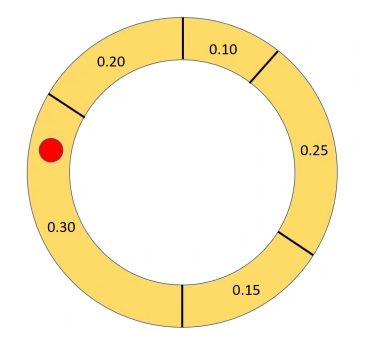
\includegraphics[width=8cm]{images/rulet.png}
\caption{Proporcionalna selekcija roditelja.}
\label{fig:rulet}
\end{figure}

Veliki brojevi predstavljaju problem, kod populacije s 5 rasporeda od kojih nakon transformacije svi imaju redom vrijednosti 10001, 10002, 10003, 10004 i 10005 razlike vjerojatnost svakog rasporeda će biti zanemarive i svi rasporedi će efektivno imati vjerojatnost od 20\%. Kako bi se taj efekt ublažio, moguće je sve kazne iz populacije umanjiti vrijednošću za jedan manjom od najmanje vrijednosti. Tako sada redom vrijednosti iznose 1, 2, 3, 4, 5.

Sljedeći problem predstavljaju negativne vrijednosti, zbog nagrada koje rasporedi mogu poprimiti, kazna rasporeda može teoretski poprimiti negativnu vrijednost, zato je potrebno pronaći minimalnu vrijednost i u slučaju da je ta vrijednost negativna, svaki element se uveća za apsolutu vrijednost najmanje kazne.

Nadalje, vrijednosti svih kazni rasporeda u svakom krugu iteracije su skoro podjednake, stoga ako se u iteraciji nalazi veliki broj rasporeda, svaki raspored će imati podjednaku šansu da bude odabran i tako se efektivno dobije nasumični odabir.

Nadalje, boljim rasporedom se smatra onaj koji ima manje kolizija, zbog toga je teško dodijeliti ispravu vjerojatnost odabira, jedan način je da umjesto kazne se gleda broj kolizija, ali onda kada bi se broj kolizija smanjio na 0, svi rasporedi bi imali podjednaku vjerojatnost odabira.

Kada bi se sve ove adaptacije uvele u algoritam, jako bi usporio zbog velikog broja transformacija i kalkulacija prije samog odabira.

\subsection{K-turnirska selekcija}

Turnirska selekcija kao ulaz u algoritam prima parametar \emph{k} koji označava broj jedinki koji ulaze u turnir. Vrlo jednostavnim postupkom, iz populacije se nasumično odabere \emph{k} raspored nakon čega se jednostavno vrati onaj koji ima najmanji broj preklapanja ili u slučaju jednakog broja preklapanja onaj s najmanjom kaznom.

\begin{algorithm}
\caption{Proporcionalna selekcija}
\label{algo:proporcionalno}
\begin{algorithmic}
\STATE{populacija := new raspored[k]}
\WHILE{size(populacija) != k}
\STATE{jedinka := odaberiNasumicno(rasporedi)}
\IF{populacija ne sadrži jedinku}
\STATE{dodaj(populacija, jedinka)}
\ENDIF
\ENDWHILE
\STATE{roditelj := odaberiNajbolji(populacija)}
\end{algorithmic}
\end{algorithm}

Kod punjenja pomoćne populacije, potrebno je provjeravati da novo odabrani raspored se već ne nalazi u populaciji.

\begin{figure}[htb]
\centering
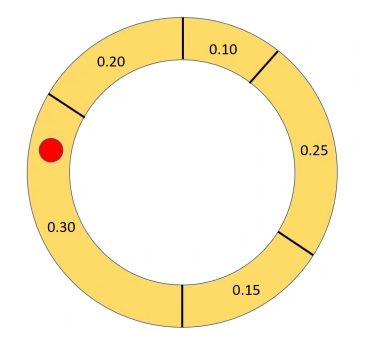
\includegraphics[width=7cm]{images/rulet.png}
\caption{Ovo ce biti turnirska selekcija.}
\label{fig:rulet}
\end{figure}

Ako se za vrijednost \emph{k} u algoritmu postavi 1, onda je to efektivno odabir nasumičnog roditelja, a ako se za \emph{k} postavi veličina populacije, onda se odabire elitna jedinka. Za broj odabranih raspored postavlja se manja vrijednost poput dvije ili tri kako bi se omogućila barem minimalno svojstvo kompetencije.

Turnirska selekcija rješava problem velikih brojeva jer odabir rasporeda ne ovisi o razlici kazni pojedinih rasporeda. Dodatno, negativne vrijednost isto ne utječu na ispravnost algoritma kao niti veliki broj rasporeda u populaciji.

Zbog svoje jednostavnosti, efikasnosti i robusnosti turnirska selekcija s parametrom tri je odabrana kao algoritam za odabir roditelja.

\section{Križanje roditelja}

Operator križanja roditelja kao i operator odabira roditelja sužuje prostor pretrage. Križanjem dvaju roditelja nastaje jedno ili dva nova rješenja  ovisno o konkretnim implementacijama. Odabrano je da operator križanja kao rezultat vraća jedno dijete. To dijete se ne odabire na osnovu svoje kazne već nasumično.

Različite implementacije daleko najmanje utječu na kvalitetu dobivenih rasporeda čak i kod ektremnih postavka operatora.

\subsection{Nasumično križanje}

Različite implementacije daleko najmanje utječu na kvalitetu dobivenih rasporeda čak i kod ekstremnih postavka operatora.

\begin{figure}[htb]
\centering
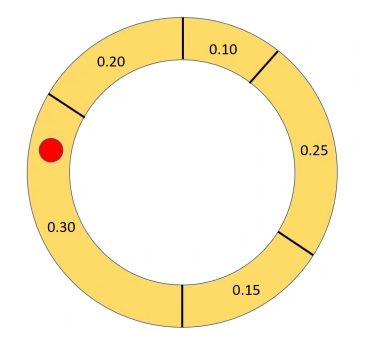
\includegraphics[width=6cm]{images/rulet.png}
\caption{Ovo ce biti turnirska selekcija.}
\label{fig:rulet}
\end{figure}

\subsection{Alternirajuće k-križanje}

Različito od nasumičnog križanja, ovdje se slučajnost odabire samo jednom, za odabir roditelja od kojeg počinje križanje. Nadalje ovisno o parametru \emph{k} koji je predan algoritmu, djetetu se postavlja idućih \emph{k} vrijednosti odabranog roditelja te s potom roditelj mijenja.

\begin{figure}[htb]
\centering
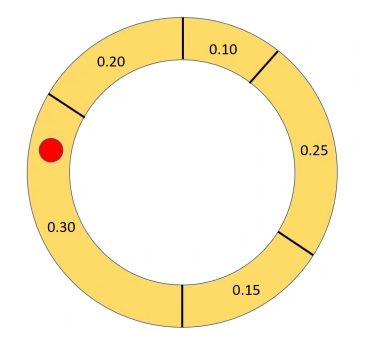
\includegraphics[width=6cm]{images/rulet.png}
\caption{Ovo ce biti turnirska selekcija.}
\label{fig:rulet}
\end{figure}

Ako se kao parametar \emph{k} postavi jedinica, onda se redom uzima termin jednog, pa termin drugog roditelja naizmjence.

\begin{figure}[htb]
\centering
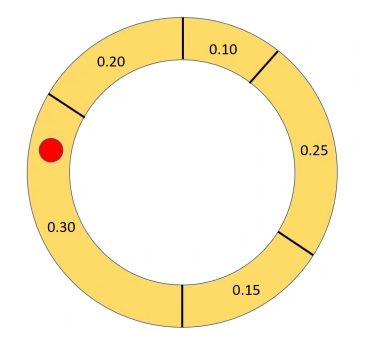
\includegraphics[width=6cm]{images/rulet.png}
\caption{Ovo ce biti turnirska selekcija.}
\label{fig:rulet}
\end{figure}

Sljedeći specijalni slučaj je ako se za parametar \emph{k} postavi vrijednost N/2, onda algoritam jednostavno uzme polovicu svakog roditelja. Također, ispravno je nazvati ovaj križanjem s polovičnom točkom prekida.

\begin{figure}[htb]
\centering
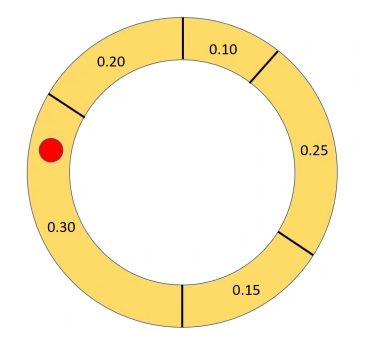
\includegraphics[width=6cm]{images/rulet.png}
\caption{Ovo ce biti turnirska selekcija.}
\label{fig:rulet}
\end{figure}

\newpage

Posljednje ako se za parametar \emph{k} odabere vrijednost veća od N/2, onda ovo postaje križanje s točkom prekida. Jedina razlika na sami algoritam križanja točkom prekida je što nisu dostupne točke prekida manje od N/2.

\begin{figure}[htb]
\centering
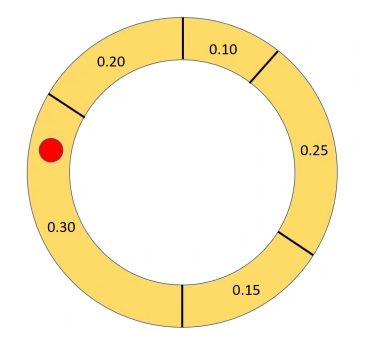
\includegraphics[width=6cm]{images/rulet.png}
\caption{Ovo ce biti turnirska selekcija.}
\label{fig:rulet}
\end{figure}

\section{Mutacija}

Osim operatora koji sužuju područje pretrage, mutacija ga proširuje. Bez operatora mutacije, vrlo brzo bi sva nova rješenja počela stagnirati, tj. ne bi dobili više novih rješenja. Operatoru je dodijeljena stopa muta, postotak studenata za koji će se promijeniti dodijeljeni termin.

Optimalna vrijednost mutacije  iznosi oko 0.002 ili 0.2\%. Raspored se sastoji od termina za 831 studenta, prema toma nakon svake mutacije će se u prosjeku promijeniti grupa za 1.66 studenta što pruža dovoljno jako svojstvo širenja. Uz veće vrijednosti konvergencija je sporija a rješenja nisu bolja.

Kod ovog problema, nije potrebno pronaći najbolje moguće rješenje već dovoljno dobro. Zato i s jako malim stopama promjene kad algoritam ima veću vjerojatnost zapeti u lokalnom optimumu to ne predstavlja problem.

\subsection{Promjena termina za fiksan broj mjesta}

Jedna od varijanti mutacije je promjena termina za fiksan broj mjesta. Na primjer studenta se prebaci s termina 8 na termin 11.

\begin{figure}[htb]
\centering
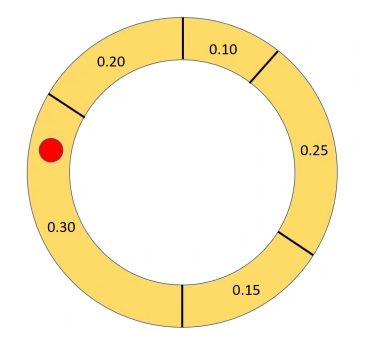
\includegraphics[width=6cm]{images/rulet.png}
\caption{Ovo ce biti turnirska selekcija.}
\label{fig:rulet}
\end{figure}

Ovako definiran operator kasnije u ciklusu pretrage kad se raspored stabilizira i većina termina imaju popunjen kapacitet od 15 ili 16 mjesta može napraviti više štete nego koristi. Ako se napravi promjena termina za 2 studenta, pogotovo ako su oni u istoj grupi, novi raspored će vrlo vjerojatno imati veću kaznu.

\subsection{Nasumičan odabir termina}

Nasumičan odabir termin radi tako da se studentu dodijeli nasumično generiran broj termina između 0 i \emph{brojTermina} gdje svaki termin ima jednaku šansu biti odabran.

\begin{figure}[htb]
\centering
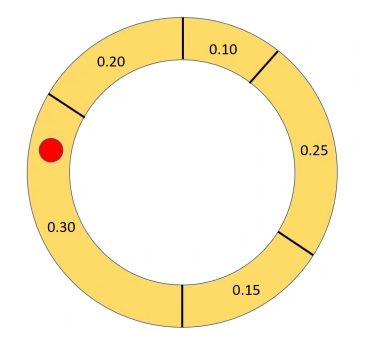
\includegraphics[width=6cm]{images/rulet.png}
\caption{Ovo ce biti turnirska selekcija.}
\label{fig:rulet}
\end{figure}

Dodjelom nasumičnog termina umjesto pomaka termina za fiksni broj mjesta bolje rješava problem potencijalnog nakupljanja termina na jednom mjestu pa je odabran kao operator mutacije.

\section{Veličina populacije}

Veličina populacije je broj rasporeda koji se u svakom trenu čuva u memoriji. S manjom veličinom populacije povećava se broj iteracija po sekundi ali je zato manja raznolikost rješenja. Pak, s većom veličinom populacije smanjit će se broj iteracija po sekundi ali će se povećati raznolikost rješenja te će se potencijalno pronaći bolje rješenje.

Operacije računanja kazne su skupe zbog velikog broja provjera kroz koje je potrebno proći, pa će se s večom populacijom broj iteracija po sekundi drastično smanjiti. Potrebno je pronači dobar balans kvalitete i brzine. Kroz testiranje vrijednosti oko 25 su se pokazale jako dobre.

\chapter{Usporedba rezultata}

Kroz rad je već izrečena odabrana konnfiguracija algorita. U ovom poglavlju će biti prikazana dodatne usporedbe rezultata zbog kojih su baš ta svojstva odabrana.

U ulaznim podacima, dostupno je više termina vježbi nego je potrebno, kod treniranja veće broja termina vidljivo je kako pno vište termina ima manji broj dodjeljenih termina, a nema gotov niti jedan termin koji ima više nego max. Kada se kazna za manji broj mjesta još više smanjima, ovaj efekt postaje akstremniji i sve je manje rasporeda koji imaju termine s popunjeni svih 16 mjesta.

Kod nagrada s većim tj. manjim vrijednostima počinju se izrazito preferirati rasporedi koji zadovoljavalju ta svojstva, čak iako se raspored smatra ``lošim''. Izrazito se usporava prolazak rasporeda s ne prekršenim ograničenjima.

Usporedba elitizma, dati primjer proporcionalnog rasporeda sa i bez elitizma.

pokazati proporciju sa velikim i malim brojem jedinki., pokazati opcenito k turnir vs proporcija.

Proporcija jako sporo konvergira k 0 zato što nema u algoirtmu kolizije

pokazati neke ekstremne situacije odabira roditelja. pokazati da i onda, rezultati su otprilike jednaki.

Pokazati primjer kada je mutacija jednaka 0

Tablice vremena dolaska do kazne: 50k, 20k, 10k, ako je populacija 10, 15, 25, 50, 150, 250

\chapter{Zaključak}
Zaključak.

\bibliography{literatura}.
\bibliographystyle{fer}

\begin{sazetak}
Ovo je sažetak mojeg rada.

\kljucnerijeci{Ključne riječi, odvojene zarezima.}
\end{sazetak}

% TODO: Navedite naslov na engleskom jeziku.
\engtitle{Creating a schedule of laboratory exercises using a genetic algorithm}
\begin{abstract}
Ovo je sažetak mojeg rada.

\keywords{Keywords, spaced apart by commas.}
\end{abstract}

\end{document}
